\begin{center}

  \begin{tabular}{rp{16cm}lp{20cm}}%{rl}

  % after \\: \hline or \cline{col1-col2} \cline{col3-col4} ...

  论文地址:& \href{https://arxiv.org/pdf/1801.07455.pdf}{https://arxiv.org/pdf/1801.07455.pdf} \\
  来源:& AAAI, 2018\\
  作者:& Sijie Yan, Yuanjun Xiong, Dahua Lin \\

  源码:& \href{https://github.com/yysijie/st-gcn}{st-gcn} \\

%  slides:& \href{http://yunshengb.com/wp-content/uploads/2017/03/nips_2018_r2l_workshop_talk.pdf}{{\footnotesize Convolutional Set Matching for Graph Similarity}}\\

  关键词:& \textbf{Action Recogonition, GCN} \\

  写于:& \date{2021-03-04}

  \end{tabular}

\end{center}

该论文\cite{yan2018spatial}针对人体动作识别问题提出了解决方案。以Skeleton为基础构建时空图,提出了ST-GCN(Spatial Temporal GCN)对人体行为的时空图进行表征,在进行行为分类。

\paragraph{问题定义}
给定一段视频,确定其中的人体行为类别。可以从多个方面表示人体行为,如光流、骨骼关键点等,该论文中采用基于骨骼关键点的形式表示人体行为。在一段视频中,每一帧中的人体骨骼点可以构成一个graph --- Spatial graph,帧与帧之间同一个骨骼点进行连接可以构成graph --- Temporal graph。论文的目标就是基于一个视频的骨骼点构成的Spatial Temporal graph来对人体行为进行分类。

\paragraph{ST-GCN思路}
\begin{figure}[h]
	\centering
	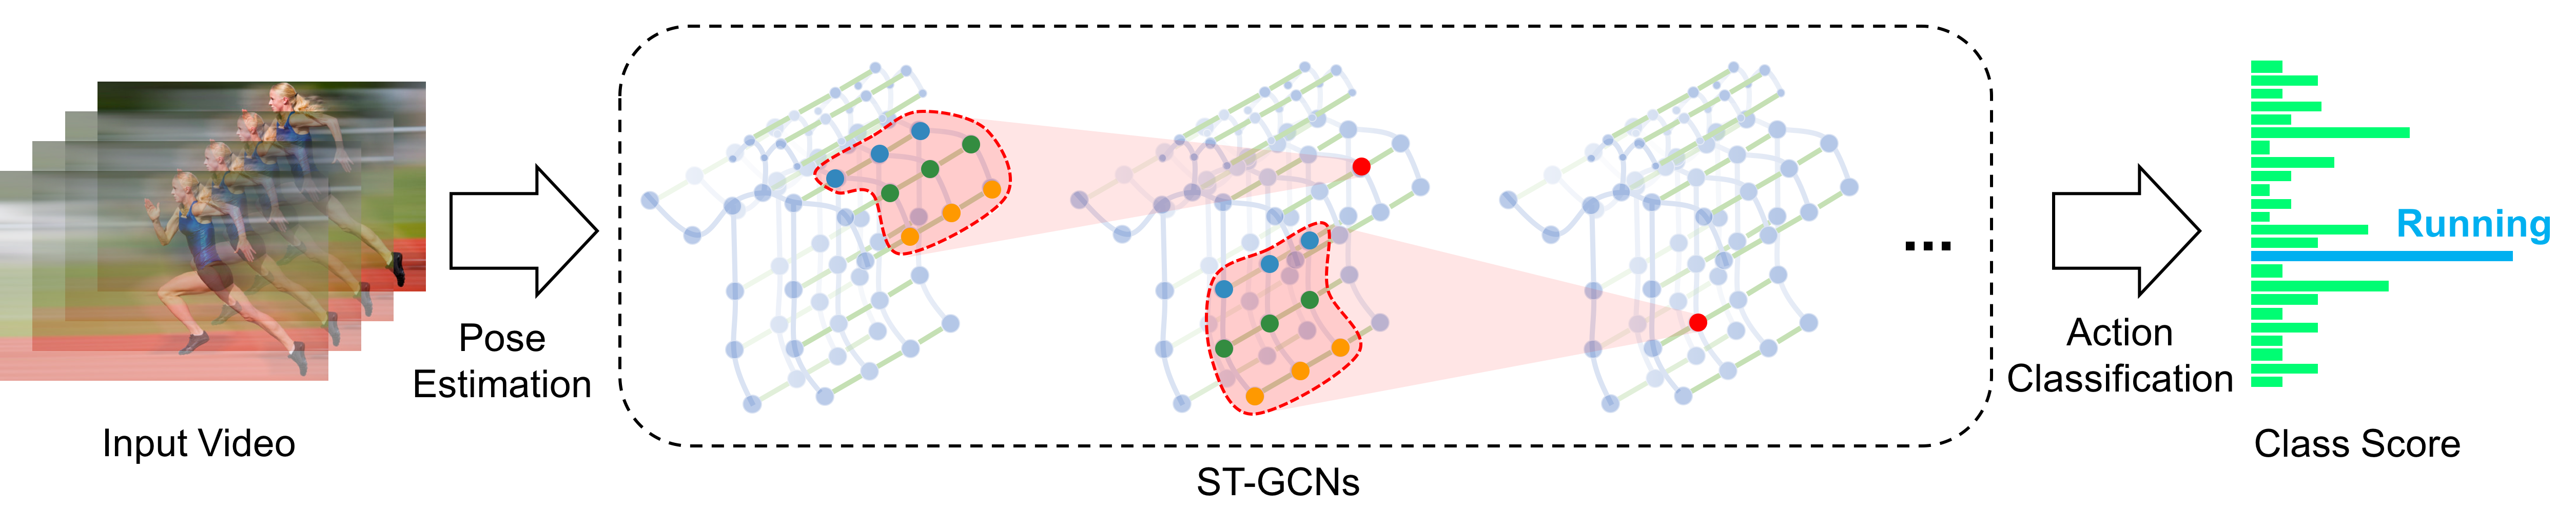
\includegraphics[width=.8\textwidth]{pics/ST-GCN.png}
	\caption{ST-GCN}
	\label{fig:st-gcn}
\end{figure}
\subparagraph{Skeleton Graph Construction}
Spatial Temporal Graph $G = (V, E)$,$V = \{v_{ti} | t=1, ..., T, i = i, ..., N\}$中的结点来自人体骨骼关键点,$N$表示关键点个数,$T$表示视频帧数。每一帧中的Graph构建以人体自然连接为依据,帧与帧之间的Graph构建方式为:相邻帧之间,同一个关键点进行相连。因此,边也分为两种:$E_S = \{v_{ti}v_{tj} | (i,j) \in H\}, E_F = \{v_{ti}v_{(t+1)i}\}$,其中$H$表示人体中关键点的自然连接。

\subparagraph{Spatial Graph Convolutional Neural Network}
作者在Spatial Temporal Graph的基础上定义了Spatial Temporal Convolution。这个卷积操作与GCN中的卷积很类似,但是加上了一个时间维度 --- 每个结点的邻居不仅要考虑当前帧中相邻的结点还要考虑时间上相邻帧的连接。对于图中每个结点,其特征为骨骼关键点在帧中的位置。

经过多层的Spatial Temporal Convolution后,将特征输入到MLP中进行行为分类即可。

\paragraph{方法解决的问题/优势}

\begin{itemize}

	\item 首次将GCN应用于行为识别
	\item 不仅考虑了帧中各个关键点,还考虑了帧间关键点

\end{itemize}

\paragraph{方法的局限性/未来方向}

\begin{itemize}

	\item 论文中提到的注意力机制没有明显的意义
	\item 只考虑了局部特征

\end{itemize}



